\documentclass[12pt,fleqn]{article}\usepackage{../common}
\begin{document}
Ders 21

Bu ozdeger/vektorler hakkindaki ilk dersimiz. Bu degerler ozel
buyukluklerdir, ozel sayilardir, ve onlari niye istedigimizi, niye
hesapladigimizi gorecegiz.

Ozvektor nedir? 

Elimde bir $A$ matrisi var. Bir matris ne yapar? Vektorler uzerinde, mesela
$x$ vektoru, etkide bulunabilir, onlari degistirebilir. Sanki $A$'yi bir
fonksiyon gibi de gorebiliriz, $x$ vektoru $A$'ya ``giriyor'' ve
``disariya'' bir $Ax$ cikiyor. Calculus'ta oldugu gibi $f()$'e bir tek sayi
$x$ veriliyor, $f(x)$ geri disari cikiyor [hakikaten de $x$ ve $Ax$ ayni
boyutta yani giris cikis analojisi cok uygun]. Lineer Cebirde daha cok
boyut var, giren ve cikan vektorler.

Bu derste ozellikle ilgilendigim vektorler ise disari ciktigi zaman girdigi
haliyle {\em ayni yonu gosteren} vektorler. Dikkat, ``ayni'' olan vektorler
degil cikinca ayni ``yonu'' gosteren vektorler. Bu tipik bir durum olmazdi
degil mi? Cogunlukla $A$'yi bir uyguladik mi disari cikan vektor tamamen
baska bir yonu gosterir. Bizim ilgilendigimiz durumda oyle olmayacak, bu
durumda $Ax$, $x$'e paralel olacak. Iste bu vektorler ozvektorler olacak. 

Paralel ne demektir? Formulle daha rahat belirtilir,

$$ Ax = \lambda x $$

$\lambda$, yani ozdeger, bir skalardir. Iki tarafta $x$'in olmasi
paralellige isaret ediyor, sadece buyukluk ($\lambda$ uzerinden) degisik
olabiliyor. Tabii buyukluk derken $\lambda$ eksi degerde olabilecegi icin
vektorun ters yonde olmasina da izin vermis oluyoruz. $\lambda$ sifir da
olabilir, hatta hayali sayi bile olabilir.

Ozdeger sifir uzerinde biraz daha duralim. Bu durumda $Ax = 0 \cdot x$ elde
ederiz yani $Ax = 0$. Bu ne demektir? $x$'lerin $A$'nin null uzayinda
(nullspace) olmasi... Eger $A$ tekil (singular) ise, ki $Ax = 0$ bu demek
zaten demek ki oyle bir $x$ olabiliyor ki $Ax = 0$ olabiliyor, o zaman $x$
sifir olmayan bir vektordur, ve $\lambda = 0$ bir ozdeger olmalidir.

Bir projeksiyon matrisine bakalim, mesela $P$. Elimizde bir satih (plane)
var, ve bu sathin uzerinde yansitma yapan bir $P$ var. 

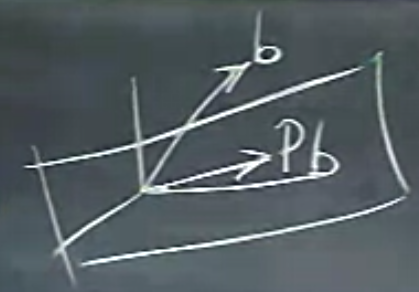
\includegraphics[height=4cm]{21_1.png}

$b$, $P$'nin bir ozvektoru mudur? Degildir. Cunku $b$ ve $Pb$ ayni yonu
gostermiyorlar. 

Peki, bu resme gore, yansitma sonrasi ayni yonde olacak bir vektor var
midir? Varsa nerededir? Cevap, eger $x$ ustteki duzlemde ise $P$ yansitmasi
sonrasi ayni yonde kalir. Tabii yansitma tekrar kendisini verir, yani
vektor hic degismemis olur. $Px = x$, ki $\lambda = 1$. 

Baska bir ozvektor var mi? Olmasini umuyorum cunku 3 boyuttayim ve bu
demektir ki 2 tane daha birbirinden bagimsiz ozvektor bulabilmeliyim, ki
nihayetinde ozcektorlerin ikisi duzlem uzerinde, ucuncusu duzlem disinda
olacak. Duzlem disinda olan ozvektor dik olan ozvektordur. 

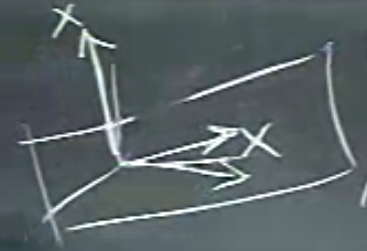
\includegraphics[height=4cm]{21_2.png}

Bu durumda $Px = 0$, ve $\lambda = 0$. 

















\end{document}
